% File content starts here - NO preamble

\section{Lower-Bound Tools}
\label{sec:lower-bound-tools}

\begin{remark}[Preconditions for This Section]
All results in this section assume the \textbf{restricted regime}: deterministic computation, single pass over input, no advice strings, no randomness. All introspection functions $\iota_d$ follow the specification in Table~\ref{tab:iota-spec} with fixed parameter $c \geq 1$ throughout.
\end{remark}

These three fundamental tools constitute the core methodology for establishing lower bounds in the restricted regime. The Budget Lemma provides a basic counting argument for transcript limitations. The $\Psi$-Fooling Bound extends this to worst-case distinguishability, while the $\Psi$-Fano Bound handles average-case scenarios with error tolerance. Together, they form the foundation for proving separations in subsequent target languages (v0.8.3--v0.8.4).

\begin{lemma}[Budget Lemma]
\label{lem:budget}
Assumes the restricted regime (deterministic, single pass, no advice, no randomness) and uses Table~\ref{tab:iota-spec}.
For any Psi-TM with introspection depth $d \geq 1$, running for $T \geq 1$ steps on input of length $n \geq 1$, where the introspection function $\iota_d$ (Table~\ref{tab:iota-spec}) exposes at most $B(d,n) = c \cdot d \cdot \log n$ bits per step with fixed parameter $c \geq 1$:
\begin{equation}
\label{eq:budget-bound}
\text{Number of distinct transcripts} \;\leq\; 2^{\,T\,\cdot\, B(d,n)}
\end{equation}
This bound is tight in the worst case.
\end{lemma}

\begin{proof}[Proof sketch]
A \textbf{transcript} is the sequence $(y_1, y_2, \ldots, y_T)$ where $y_t = \iota_d(C_t, n)$ is the introspection output at step $t$ and $C_t$ is the machine configuration. Each step exposes at most $B(d,n)$ bits via $\iota_d$. Over $T$ steps, total information $\leq T \cdot B(d,n)$ bits. Number of possible transcript sequences $\leq 2^{T \cdot B(d,n)}$.

\textbf{Tightness:} This bound is achieved when $\iota_d$ outputs the maximum allowed payload at each step. For example, consider the introspection function:
\[
\iota_d(C_t, n) \;=\; \text{encode}\big(\text{step\_number}(t) \;\|\; \text{head\_position}(C_t) \;\|\; \text{state}(C_t)\big)
\]
where the encoding uses exactly $B(d,n)$ bits by padding or truncating as needed. Over $T$ steps, this produces $2^{T \cdot B(d,n)}$ distinct transcript sequences when the machine visits $2^{B(d,n)}$ different configurations per step.

This differs from classical transcript counting by the explicit $B(d,n)$ constraint from Table~\ref{tab:iota-spec}.
\end{proof}

\begin{lemma}[\(\Psi\)-Fooling Bound]
\label{lem:psi-fooling}
Assumes the restricted regime and uses Table~\ref{tab:iota-spec}.
For any deterministic Psi-TM with introspection depth $\leq d$, input length $n \geq 1$, running time $T \geq 1$, and fooling set $\mathbb{F}_n$ with $|\mathbb{F}_n| = M \geq 2$ pairwise distinguishable inputs, where introspection function $\iota_d$ (Table~\ref{tab:iota-spec}) provides at most $B(d,n) = c \cdot d \cdot \log n$ bits per step:
\begin{equation}
\label{eq:fooling-bound}
T \;\geq\; \left\lceil \frac{\log M}{B(d,n)} \right\rceil
\end{equation}
\end{lemma}

\begin{proof}[Proof sketch]
By Lemma~\ref{lem:budget}, after $T$ steps there are at most $2^{T \cdot B(d,n)}$ distinct transcripts. To distinguish $M$ inputs in the fooling set, require $2^{T \cdot B(d,n)} \ge M$, hence $T \cdot B(d,n) \ge \log M$ and the bound follows by ceiling. Classical fooling arguments use unlimited communication; here the channel capacity is bounded by $B(d,n)$ bits per step.
\end{proof}

\begin{lemma}[\(\Psi\)-Fano Bound]
\label{lem:psi-fano}
Assumes the restricted regime and uses Table~\ref{tab:iota-spec}.
For any Psi-TM with introspection depth $\leq d$, input length $n \geq 1$, running time $T \geq 1$, input distribution over $M \geq 2$ outcomes, and error probability $0 < \varepsilon < 1 - 1/M$, where introspection function $\iota_d$ (Table~\ref{tab:iota-spec}) provides channel capacity $T \cdot B(d,n)$ bits with $B(d,n) = c \cdot d \cdot \log n$:
\begin{equation}
\label{eq:fano-bound}
T \;\geq\; \frac{\log M - h(\varepsilon) - \varepsilon\,\log(M-1)}{B(d,n)}
\end{equation}
where $h(\varepsilon) = -\varepsilon \log \varepsilon - (1-\varepsilon) \log(1-\varepsilon)$ is the binary entropy.
\end{lemma}

\begin{proof}[Proof sketch]
Standard Fano's inequality applies to transcript information with mutual information measured in bits. This follows the standard form of Fano's inequality: $H(X\mid Y) \leq h(\varepsilon) + \varepsilon \, \log(|X|-1)$ where $X$ is the input distribution and $Y$ is the observed transcript. The machine observes $\leq T \cdot B(d,n)$ bits total, providing channel capacity $T \cdot B(d,n)$. Hence $T \cdot B(d,n)$ must be at least $\log M - h(\varepsilon) - \varepsilon \log(M-1)$. Classical Fano's inequality uses arbitrary channel capacity; here adapted to the $B(d,n)$ constraint specific to $\Psi$-TM with introspection depth $d$.
\end{proof}

\subsection{Worked Examples}
\subsubsection{Example Application}
The following illustrates Lemma~\ref{lem:psi-fooling} in action.

Consider depth $d = 2$, input length $n = 1000$, with fixed parameter $c = 1$ throughout.
Thus $B(2,1000) = 1 \cdot 2 \cdot \log 1000 \approx 2 \cdot 10 = 20$ bits per step.

For a fooling set of size $M = 2^{100}$ (i.e., $|\mathbb{F}_n| = 2^{100}$): by equation~\eqref{eq:fooling-bound},
\[T \;\geq\; \left\lceil \frac{\log M}{B(d,n)} \right\rceil = \left\lceil \frac{100}{20} \right\rceil = 5 \text{ steps}\]

This demonstrates that any depth-2 $\Psi$-TM requires at least 5 computation steps to distinguish between $2^{100}$ carefully constructed inputs, regardless of algorithmic sophistication.

\begin{remark}[Dependency Structure]
These tools form a hierarchy of increasing specificity:
\begin{itemize}
\item \textbf{Budget Lemma} $\to$ fundamental counting (base for all arguments)
\item \textbf{$\Psi$-Fooling Bound} $\to$ worst-case distinguishability (enables UB/LB proofs)
\item \textbf{$\Psi$-Fano Bound} $\to$ average-case information theory (handles probabilistic scenarios)
\end{itemize}
\end{remark}

\subsubsection{Example Application (Average-Case)}
The following illustrates Lemma~\ref{lem:psi-fano} for average-case analysis.

Consider the same parameters: depth $d = 2$, input length $n = 1000$, so $B(2,1000) = 20$ bits per step.

Suppose we have a uniform distribution over $M = 2^{60}$ possible inputs, and we want error probability $\varepsilon = 0.1$ (10\% error rate). The binary entropy is:
\[h(0.1) = -0.1 \log(0.1) - 0.9 \log(0.9) \approx 0.469 \text{ bits}\]

By Lemma~\ref{lem:psi-fano}:
\begin{align}
T &\geq \frac{\log M - h(\varepsilon) - \varepsilon \log(M-1)}{B(d,n)} \\
&\geq \frac{60 - 0.469 - 0.1 \cdot 60}{20} \\
&\geq \frac{60 - 0.469 - 6}{20} = \frac{53.531}{20} \approx 2.68
\end{align}

Therefore $T \geq 3$ steps. This shows that even allowing 10\% error rate, any depth-2 $\Psi$-TM needs at least 3 steps to distinguish inputs from this distribution, demonstrating the power of information-theoretic arguments in average-case scenarios.

\subsubsection{Example Application (High-Depth Case)}
Consider higher depth $d = 3$, larger input $n = 2^{20} = 1{,}048{,}576$, with $c = 1$.
Thus $B(3,2^{20}) = 3 \cdot \log(2^{20}) = 3 \cdot 20 = 60$ bits per step.

For fooling set $M = 2^{900}$:
\begin{equation}
T \geq \left\lceil \frac{900}{60} \right\rceil = 15 \text{ steps}
\end{equation}

This demonstrates scalability: even with a significantly higher introspection budget (60 vs 20 bits), a proportionally larger fooling set still forces meaningful time complexity.

\begin{remark}[Comparison: Worst-Case vs Average-Case]
\par\smallskip
\begin{center}
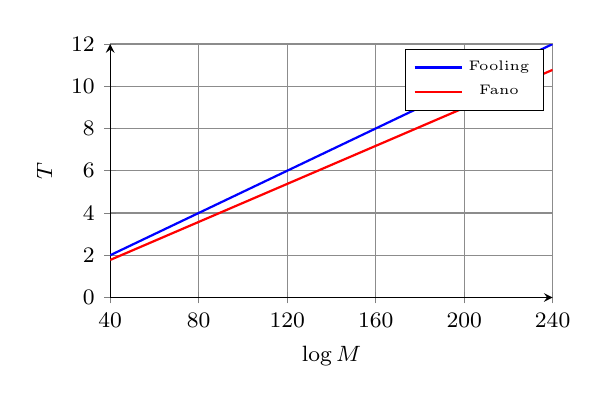
\begin{tikzpicture}[scale=1.0]
\begin{axis}[
    width=7.2cm, height=4.8cm,
    grid=both,
    major grid style={draw=black!45},
    minor grid style={draw=black!20},
    axis lines=left,
    ticks=both,
    xlabel={\footnotesize $\log M$},
    ylabel={\footnotesize $T$},
    xmin=40, xmax=240,
    ymin=0, ymax=12,
    xtick={40,80,120,160,200,240},
    ytick={0,2,4,6,8,10,12},
    tick label style={font=\footnotesize},
    label style={font=\footnotesize},
    legend style={font=\scriptsize}
]
\addplot[blue, thick, domain=40:240, samples=200] {x/20};
\addlegendentry{\tiny Fooling}
\addplot[red, thick, domain=40:240, samples=200] {(0.9*x - 0.469)/20};
\addlegendentry{\tiny Fano}
\end{axis}
\end{tikzpicture}
\end{center}

\noindent\begin{minipage}{0.96\textwidth}
\textbf{Compare the two approaches:}
\begin{itemize}[leftmargin=1.2em]
\item Fooling set: $M = 2^{100} \Rightarrow T \ge 5$ steps (worst-case)
\item Fano bound: $M = 2^{60},\ \varepsilon = 0.1 \Rightarrow T \ge 3$ steps (average-case)
\end{itemize}
The Fano bound trades input complexity for error tolerance, typically yielding weaker but more general bounds.
\end{minipage}
\end{remark}

\begin{table}[h]
\centering
\caption{Summary of Lower-Bound Tools (assumes restricted regime \& Table~\ref{tab:iota-spec} budget)}
\label{tab:lower-bound-summary}
\small
\begin{tabular}{@{}p{2.5cm}p{5.5cm}p{3cm}p{3.5cm}@{}}
\toprule
\multicolumn{4}{c}{\textbf{Key Formula: } $B(d,n) = c \cdot d \cdot \log n$} \\
\midrule
Lemma & Statement & Proof Idea & Usage \\
\midrule
Budget Lemma & $\leq 2^{T \cdot B(d,n)}$ transcripts & Counting argument & All target languages \\
$\Psi$-Fooling Bound & $T \geq \lceil \log M / B(d,n) \rceil$ & Distinguishability & Pointer-chase $L_k$ \\
$\Psi$-Fano Bound & $T \geq [\log M - h(\varepsilon) - \varepsilon \, \log(M-1)] / B(d,n)$ & Fano's inequality & Average-case analysis \\
\bottomrule
\end{tabular}
\end{table}

\begin{remark}[Visualization]
Figure~\ref{fig:bounds-visualization} shows the linear relationship between transcript requirements $T$ and fooling set size $\log|\mathbb{F}_n|$ for different budget constraints $B(d,n)$.
\end{remark}

\begin{figure}[htbp]
\centering
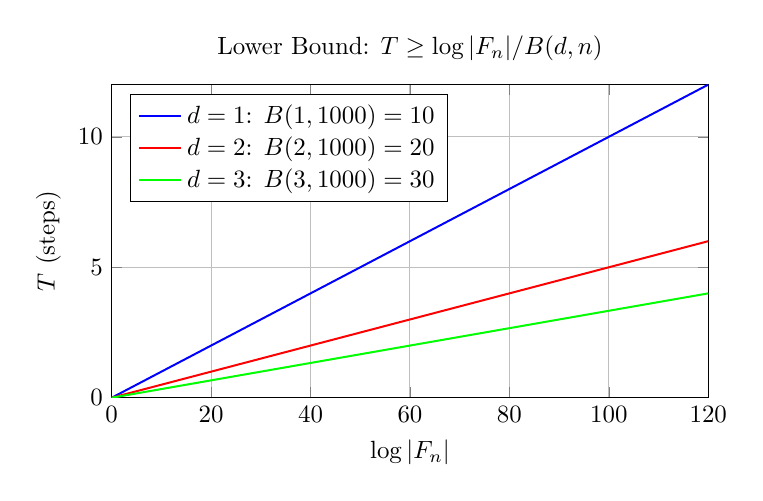
\begin{tikzpicture}[scale=0.9]
\begin{axis}[
    width=10cm, height=6cm,
    xlabel={$\log|\mathbb{F}_n|$},
    ylabel={$T$ (steps)},
    xmin=0, xmax=120,
    ymin=0, ymax=12,
    grid=major,
    legend pos=north west,
    title={Lower Bound: $T \geq \log|\mathbb{F}_n| / B(d,n)$}
]
% d=1, n=1000: B(1,1000) ≈ 10
\addplot[blue, thick, domain=0:120, samples=200] {x/10};
\addlegendentry{$d=1$: $B(1,1000) = 10$}

% d=2, n=1000: B(2,1000) ≈ 20  
\addplot[red, thick, domain=0:120, samples=200] {x/20};
\addlegendentry{$d=2$: $B(2,1000) = 20$}

% d=3, n=1000: B(3,1000) ≈ 30
\addplot[green, thick, domain=0:120, samples=200] {x/30};
\addlegendentry{$d=3$: $B(3,1000) = 30$}
\end{axis}
\end{tikzpicture}
\caption{Equation~\eqref{eq:fooling-bound}: Time complexity grows linearly with fooling set size, inversely with introspection budget}
\label{fig:bounds-visualization}
\end{figure}

\begin{figure}[htbp]
\centering
\begin{tikzpicture}[node distance=2cm, every node/.style={align=center, minimum width=2.5cm}]

% Input layer
\node[rectangle, draw, fill=blue!20, thick] (input) {Input Space\\$|\mathbb{F}_n| = M$};

% Budget layer  
\node[rectangle, draw, fill=yellow!30, above of=input] (budget) {Budget Lemma\\Eq.~\eqref{eq:budget-bound}\\$\leq 2^{T \cdot B(d,n)}$ transcripts};

% Bounds layer
\node[rectangle, draw, fill=green!30, above left of=budget, xshift=-1cm] (fooling) {Fooling Bound\\Eq.~\eqref{eq:fooling-bound}\\Worst-case};
\node[rectangle, draw, fill=orange!30, above right of=budget, xshift=1cm] (fano) {Fano Bound\\Eq.~\eqref{eq:fano-bound}\\Average-case};

% Result layer
\node[rectangle, draw, fill=red!20, above of=budget, yshift=2cm] (result) {Lower Bound\\$T = \Omega(\log M / B(d,n))$};

% Arrows
\draw[->, thick, blue] (input) -- (budget);
\draw[->, thick, green] (budget) -- (fooling);
\draw[->, thick, orange] (budget) -- (fano);
\draw[->, thick, green] (fooling) -- (result);
\draw[->, thick, orange] (fano) -- (result);

% Labels on arrows
\node[above, rotate=35] at ($(budget)!0.5!(fooling)$) {\small distinguishability};
\node[above, rotate=-35] at ($(budget)!0.5!(fano)$) {\small error probability};

\end{tikzpicture}
\caption{Complete derivation flow: from input complexity through transcript bounds to time lower bounds}
\label{fig:lower-bound-mechanism}
\end{figure}

These information-theoretic bounds enable the separation proofs in Section~\ref{sec:target-languages}. For the pointer-chase language $L_k$ in v0.8.3, we will construct fooling sets with $M = 2^{\alpha m}$ where $m = \Theta(n/k)$, yielding:
\begin{equation}
\label{eq:lk-preview}
T(n) = \Omega\!\left(\frac{\alpha \cdot n/k}{(k-1) \cdot \log n}\right) = \Omega\!\left(\frac{n}{k(k-1)\log n}\right)
\end{equation}
by applying equation~\eqref{eq:fooling-bound} at depth $k{-}1$. The upper bound construction achieves $O(n)$ time at depth $k$ through sequential table lookups, establishing the strict separation $L_k \in \text{Psi-P}_k \setminus \text{Psi-P}_{k-1}$.

